\begin{figure*}
\captionsetup{width=0.25\linewidth,justification=raggedright}
\begin{minipage}[t]{0.3\linewidth}
\begin{center}
\includegraphics[width=\textwidth,height=1.7\textwidth]{figure/k3pd_k3pv_z1_note.eps}
\end{center}
\vspace{-0.7cm}
\caption{
    Illustrating how different scales of density and velocity 
    fields contribute to kSZ signal at $\ell\sim 500-3000$. 
    Red lines circle the most essential modes. 
}
\label{fig:k3v}
\end{minipage}
\begin{minipage}[t]{0.3\linewidth}
\begin{center}
\includegraphics[width=\textwidth,height=1.7\textwidth]{figure/powv2d_z1z2_r15r10.eps}
\end{center}
\vspace{-0.7cm}
\caption{The correlation coefficient between reconstructed $v_z$  and actual $v_z$ 
assuming a baseline of 100m, foregrounds 
    smear $k_z$ below $~0.08$ h/Mpc and $~0.12$ h/Mpc 
    at $z=1,2$ respectively. }
\label{fig:v}
\end{minipage}
\begin{minipage}[t]{0.3\linewidth}
\begin{center}
\includegraphics[width=\textwidth,height=1.7\textwidth]{figure/powmomen_before_after_tide.eps}
\end{center}
\vspace{-0.7cm}
\label{fig:p}
\caption{The correlation coefficient for $p_\parallel=(1+\delta)v_z$ before and 
after tidal reconstruction. 
The kSZ is roughly $p_\parallel$ integrated over line of sight, 
corresponding to $k_z=0$ modes.}
\end{minipage}
\end{figure*}
To search for compensations, 
it is important to pinpoint the missing modes for generating kSZ signals. 

The first step is to clarify which angular scale of the kSZ signal 
we are interested in. 
As demonstrated in Fig.\ref{fig:cmb_21cm}, 
the kSZ effect is too faint to 
be distinguished until 
primary CMB starts to fade away, 
which is roughly $\ell>500$. 
It is possible to select a frequency band with thermal SZ signal negligible, 
then the dominate factor on high $\ell$ will be the CMB facility noises. 
Consider existing Planck \cite{Planck2015} data at 217 GHz, 
$\ell \sim 500-3000$ will be the visible window for kSZ signal. 
The window could be extended to higher frequency with 
ACTpol and CMB-S4. 


The next step is to understand what role each scale plays in generating kSZ signal 
at $\ell \sim 500-3000$. 
Write Eq.(\ref{eq:ksz}) in Fourier space. 
Given $g(\eta)$ varies slowly. 
$\Theta(\bm{\ell})$ is propotional to the $k_z=0$ mode of the momentum field, as marked in Fig.\ref{fig:p}, 
%$p_\parallel(\bm{k})$. 
\begin{eqnarray}
    \label{eq:thetak}
    \Theta(\bm{\ell})&\propto&p_\parallel({k}_x\chi,{k}_y\chi,0)\\
    &\propto&\int 
    d^3k^\prime\,\delta(\bm{\ell}/\chi-\bm{k}_\perp^\prime,k_\parallel^\prime) v_z(\bm{k^\prime})\nonumber
    \end{eqnarray}

The convolution of $\delta$ and $v_z$ 
indicates the signal comes from the cross talk of 
$\bm{\ell}/\chi-\bm{k}_\perp^\prime$ and $\bm{k}_\perp$, 
sum over all $k^\prime$. 

Since $v_z \propto k_z/k^3$, 
it drops fast at small scales. 
Boldly analogize $v_z$ to a Dirac delta function $\delta^D(\bm{k}^\prime)$, 
$\Theta(\bm{\ell})$ will reduce to $\propto\delta(\bm{\ell}/\chi,0) v_z(0,0)$, 
with integration of other $k^\prime$ negligible due to the faintness of 
$v_z(k^\prime\neq0)$. 
Adapt the analogy into reality, 
where $v_z(\bm{k})$ 
is not as sharp as $\delta^D$, 
and the peak will be more close to 
($k_\perp$,$k_\parallel$)=($0.01$,$0.1$) h/Mpc 
rather than (0,0),
we will see  
that most of the kSZ signals are 
generated from the cross talk between the part of 
$v_z(\bm{k})$ with k in a small ball  
surrounding (0.01,0.1) h/Mpc 
and the part of $\delta(k)$ with k close to 
$\delta(\bm{\ell}/\chi,0.1)$ h/Mpc. 
This is demonstrated in Fig.\ref{fig:k3v}. 
%Background color indicates the contribution of $|\delta(k)|$ and $|v_z(k)|$ 
%during Fourier transform. 
Comparing it with Fig.\ref{fig:cmb_21cm}, 
we notice that while the 
essential modes for $\delta$ are partly resolved, 
the large scale information dominating $v_z$ is 
almost completely drained out in 21 IM fields.

Therefore, the primary task to restore the cross correlation 
between kSZ and 21cm IM fields is to reconstruct the 
large scale modes for $v_z$.
